Doom development started around XXX. While 
 \begin{figure}[H]
\centering  
\begin{tabularx}{\textwidth}{ X  X  X  }
  \toprule
  \textbf{Name} &  \textbf{Age} & \textbf{Occupation} \\
  \toprule 
   John Carmack & 22 &  Programming\\
   John Romero & 26 &  Programming\\
   Adrian Carmack & 23 &  Artist\\
   Tom Hall & 29 &  Creative Director\\
   Jay Wilbur & 31 &  Business\\
   Kevin Cloud\protect\footnotemark & 28 &  Computer Artist\\
   Donna Jackson & ?? & id's Mom\\
     \toprule
\end{tabularx}
\caption{id Software at the start of Doom development.}\label{fig:Id Software team}
\end{figure}
\par
Due to creative differences, Tom Halls left id around XXX. Six people were hired. Blabl blab
 \begin{figure}[H]
\centering  
\begin{tabularx}{\textwidth}{ X  X  X  }
  \toprule
  \textbf{Name} &  \textbf{Age} & \textbf{Occupation} \\
  \toprule 
   Dave Taylor & ?? & Programming\\
   Sandy Petersen & 39 & Designer\\
   Shawn Green & ?? & Software Support\\
   American McGee & 22 & Tech Support\\
   Paul Radek & 28 & ??\\
   Gregor Punchatz & 27 & Artist\\
     \toprule
\end{tabularx}
\caption{id Software recruits for Doom.}\label{fig:Id Software team}
\end{figure}

\trivia{Gregor is the son of Don Ivan Punchatz, who created the Doom package art and logo.}\\
\par

\trivia{The credit screen evolved with each beta version of Doom. Notice how NeXT computer were originally credited, witnessing how important the development machine were to id. In version 1.25, Michael Abrash (who would only join id for Quake) was credited due to the quality of his article in XXX and Graphic Black Book ???.}\\
\par
\cscaledimage{0.9}{credits/DoomCREDIT10.png}{v1.0}
\par
\cscaledimage{0.9}{credits/DoomCREDIT19.png}{v1.1 to v1.9}
\par
\cscaledimage{0.9}{credits/DoomCREDIT125.png}{v1.25}
\par
\cscaledimage{0.9}{credits/DoomCREDITUD.png}{Ultimate Doom}
\par
\par
\begin{minipage}{1.0\textwidth}
\par
\fullimage{idsoftware_crew.png}
\par




% One cool page :) !
\begin{minipage}{.6\textwidth}
In January of 1995, Electronic Games magazine ran a serie of three articles for the released of Doom II. An opportunity to gather all members of id team in the group photo shown above. In the back row, left to right: Kevin Cloud, American Mcgee, John Carmack, Adrian Carmack, Sandy Petersen. Front row: Dave Taylor, John Romero and Shawn Green.\\
\par
The plank in the photo is in fact John Romero's office door. The hole in it is the making of John Carmack involving what John Romero is holding in the photo on the right.\\
\end{minipage}
\begin{minipage}{.4\textwidth}
\centering
\scaledimage{0.95}{johns_weapons.png}
\par
\end{minipage}

\par
\fq{Well, Romero's doom jammed one day. He was in his office and was trapped in there,
and we couldn't get the door open. It was after-hours, so we couldn't call building
maintenance, and we were all standing around trying to figure out what to do, when
it occured to me and I said, "You know, I do have a batle axe in my office."\\
\par
Yes, this thing really works.}{John Carmack}
\end{minipage}



\section{Organization}
\par
TODO: Map
\par
\fullimage{palette.png}
\par
\fullimage{colormap.png}

\par

 Town East Tower in Mesquite, near Big Billy Barren's Used Cars and Sheplers Western Store. The black cube.
\par
\begin{figure}[H]
\centering
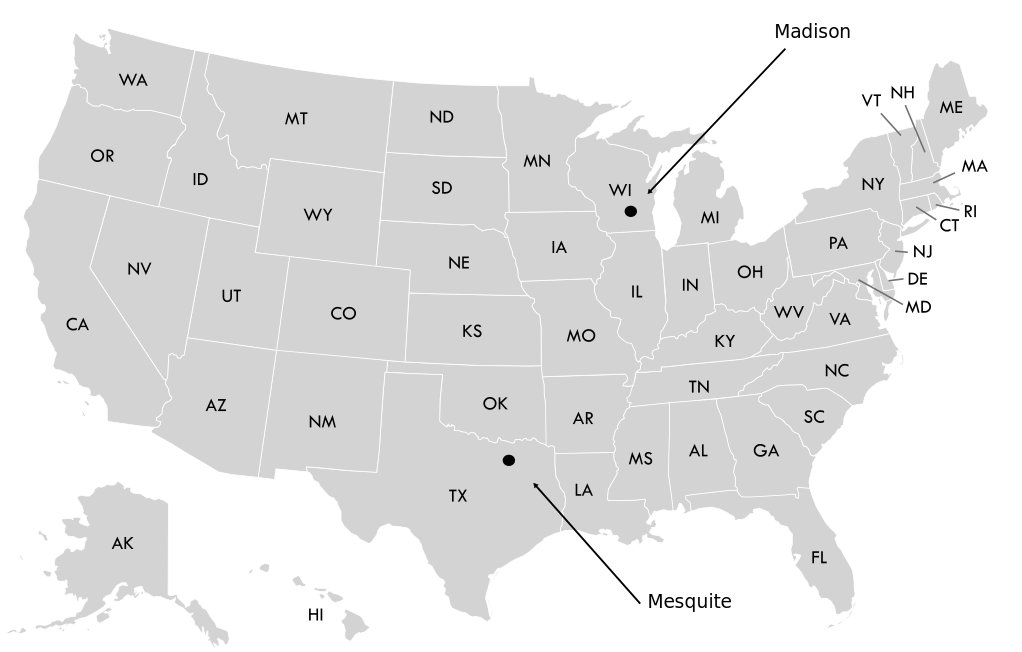
\includegraphics[width=\textwidth]{drawings/usa-id-software.pdf}
\end{figure}
\par

\fq{On the first day. each guy chose his space. Carmack and Romero took side-by-side offices, while Adrian and Kevin, who were growing increasingly close, decided to share a space. Tom liked an open corner spot in a large room with a window. "This would be a great office area," he said, "we just need to put some walls up." The rest agreed. But the walls were slow to come. When- ever Tom asked Jay about it, Jay would say they were on their way. Out of humor and frustration, Tom put down two long strips of masking tape where the walls of what he called his creative corner would go.}{David Kushner, Masters of Doom}
\par
\begin{figure}[H]
\centering
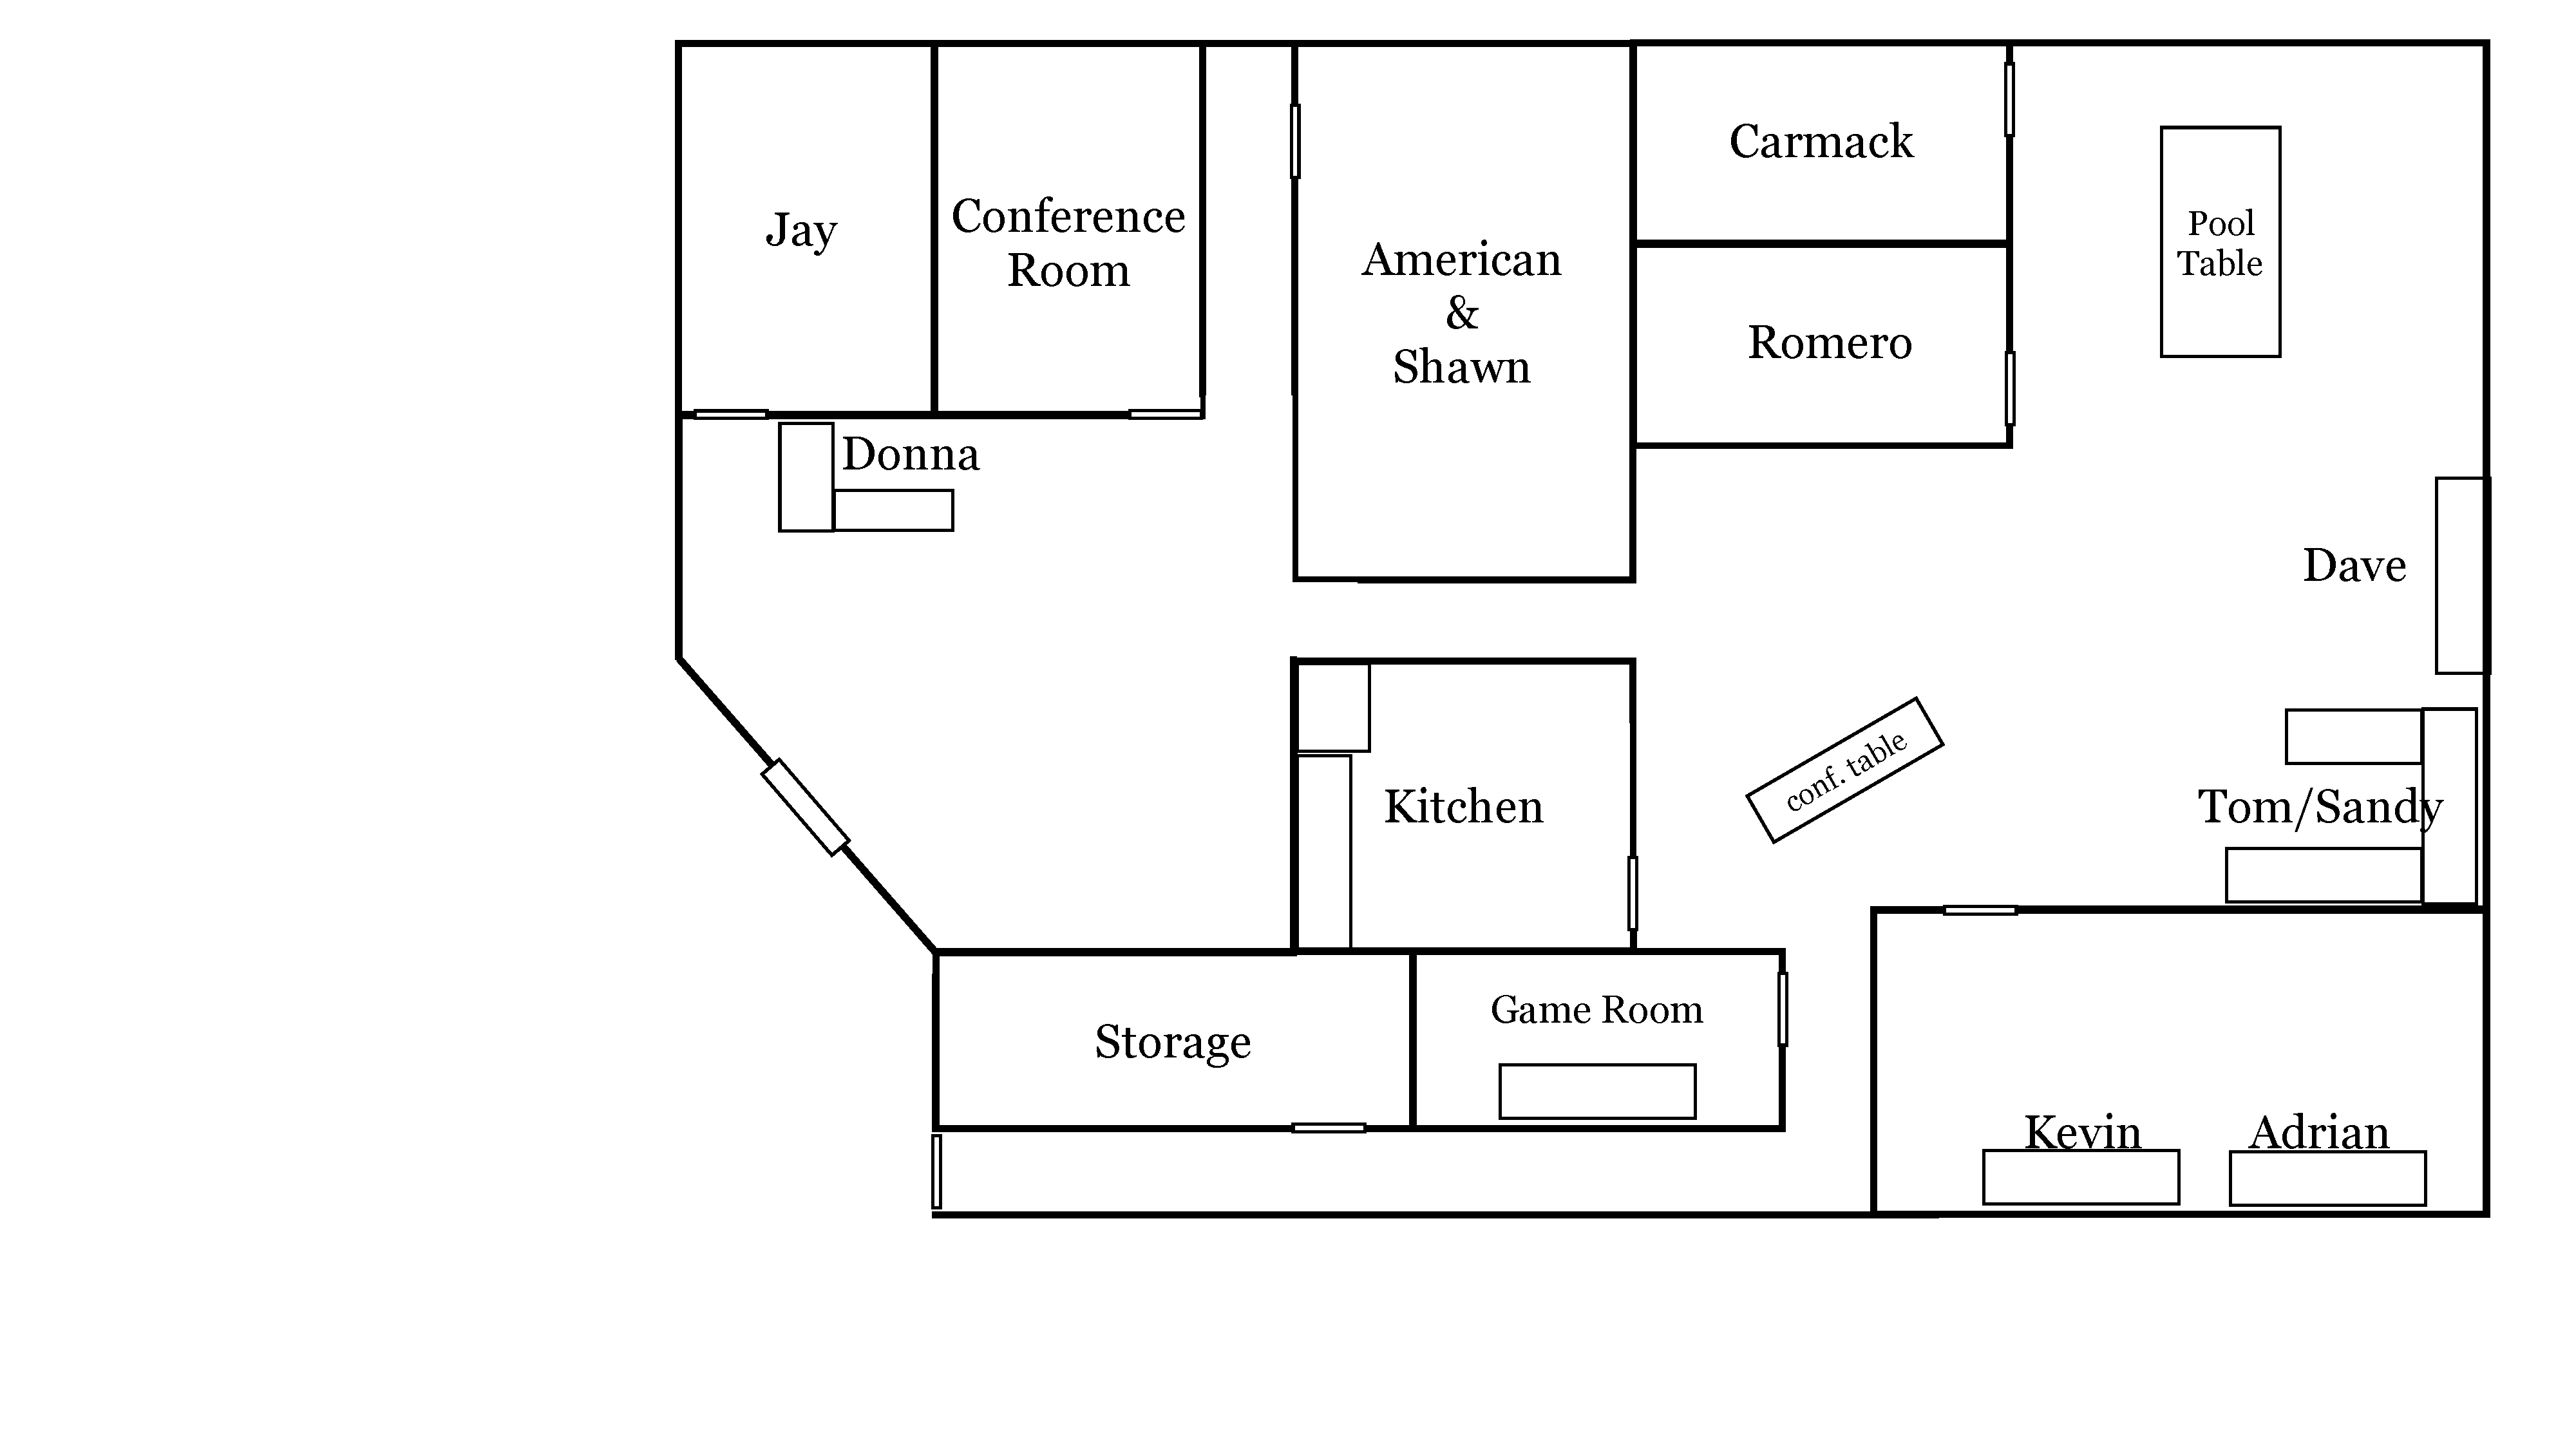
\includegraphics[width=\textwidth]{drawings/id-software-office-mesquite.pdf}
\end{figure}
\par

\section{DoomED}
\fullimage{doomed/DoomEd.png}
\par
\fullimage{doomed/all_widgets.png}
\par
\tcode{cloc_doomed.txt}
\par
\tcode{map.txt}

\section{doombsp}
\cw{doombsp} processes output from DoomED (XXX files) into XXX, XXX, and XXX. It was released very shorty after Doom shareware on April, 6th 1994. It is a small code base which was critical to the modding community since it enabled enthousiast to compile and inject their own maps into Doom.\\
\par
\tcode{cloc_doombsp.txt}
\par
Trivia: WAD was coined by Tom Halls. "Where's all the data?".
\section{Scanning tools}
\par
Screenshots running:\\
\par

\section{Backgrounds}
bla

Doom 1 backgrounds:\\
\par
\scaledimage{0.9}{skies/doom/SKY1.png}\\
\scaledimage{0.9}{skies/doom/SKY2.png}\\
\scaledimage{0.9}{skies/doom/SKY3.png}\\

Ultimate Doom episode 4 background:\\
\par
\scaledimage{0.9}{skies/ultimate_doom/SKY4.png}

Doom 2 backgrounds:\\
\par
\par
\scaledimage{0.9}{skies/doom2/RSKY1.png}\\
\scaledimage{0.9}{skies/doom2/RSKY2.png}\\
\scaledimage{0.9}{skies/doom2/RSKY3.png}\\

Doom TNT changed the way background were handled. Instead of one bitmap, four were used:\\



\begin{minipage}{\textwidth}
\fullimage{skies/doom/e1m1.png}
\par
Yangshuo Cavern in China (MAJEST3.BMP, 640x480)\\
\par
\fullimage{MAJEST3.png}
\end{minipage}
\par


\begin{minipage}{\textwidth}
\fullimage{skies/doom/e2mx.png}
\par
MAJEST3.BMP, 640x480\\
\par
\fullimage{MAJEST4.png}
\end{minipage}
\par


\begin{minipage}{\textwidth}
\fullimage{skies/doom/e3m1.png}
\par
MAJEST3.BMP, 640x480\\
\par
\fullimage{WILD4.png}
\end{minipage}

\par

\begin{minipage}{\textwidth}
\fullimage{skies/doom2/e1m1.png}
\par
MAJEST3.BMP, 640x480\\
\par
\fullimage{WILD4.png}
\end{minipage}


\begin{minipage}{\textwidth}
\fullimage{skies/doom/e3m1.png}
\par
MAJEST3.BMP, 640x480\\
\par
\fullimage{WORLD2.png}
\end{minipage}


\section{Backgrounds}
Props

\section{music}
fq{“Much of what was in Doom Bible never appeared in the game, but it set a mood for starting on the project. Within a few months of receiving that document, I had roughed out a lot of music and most of what turned out to be final sound effects.”}{Bobby Prince, Retro Gamer 44.}

\section{Distribution}
\fq{We don’t care if you make money off this shareware demo,” Jay told retailers. “Move it. Move it in mass quantities.” The retailers couldn’t believe their ears, no one had ever told them not to pay royalties.
But Jay was insistent. “Take DOOM for nothing, keep the profit. My goal is distribution. DOOM is going to
be Wolfenstein on steroids, and I want it far and wide.
I want you to stack DOOM high. In fact, I want you to
do advertising for it, too, because you’re going to make money off it. So take this money that you might have given me in royalties and use it to advertise the fact that you’re selling DOOM.}{Jay}


\section{Dave Taylor Leak anecdote}
